\documentclass[12pt,a4paper]{article}
\usepackage{graphicx}
\usepackage{subcaption}
\usepackage[utf8]{inputenc}
\usepackage[T5]{fontenc}
\usepackage[top=2.5cm, bottom=2.5cm, left=2.5cm, right=2cm]{geometry}
\usepackage{fancyhdr}
\usepackage{titlesec}
\usepackage{array}
\usepackage{setspace}
\usepackage{tikz}
\usepackage{hyperref}
\usepackage{tocloft}
\usepackage{float}
\usepackage{makecell}
\usepackage{tabularx}
\usepackage{algpseudocode}
\usepackage{algorithm}
\usepackage{amsmath}
\usepackage{caption}
\usepackage{placeins}
\usepackage{rotating}
\usepackage{longtable}
\usepackage{ragged2e}
\usepackage{enumitem}
\usepackage{csquotes}
\usepackage{listings}
\usepackage{polyglossia}
\setmainlanguage{english}  % Ngôn ngữ chính
\setotherlanguage{vietnamese}    % Ngôn ngữ phụ

\setlength{\parindent}{2em}  % thụt đầu dòng 2 chữ
% \setlength{\parskip}{1em}    % cách dòng giữa các đoạn

\pagenumbering{arabic}
\pagestyle{fancy}
\fancyhf{}
\fancyhead[L]{Lab 01}
\fancyhead[C]{Introduction to Big Data}
\fancyhead[R]{CSC14118}
\renewcommand{\footrulewidth}{0.4pt}
\fancyfoot[L]{University of Science}
\fancyfoot[C]{Faculty of Information Technology}
\fancyfoot[R]{Page \thepage}

\renewcommand{\thealgorithm}{}
\titlespacing*{\section}{0pt}{1ex}{1ex}
\titlespacing*{\subsection}{0pt}{1ex}{1ex}
\titlespacing*{\subsubsection}{0pt}{1ex}{1ex}
\setlist{itemsep=1pt, topsep=1pt}

\setlength{\textfloatsep}{5pt}
\setlength{\intextsep}{5pt}
\captionsetup{skip=3pt}

\lstset{
    basicstyle=\ttfamily\small,
    breaklines=true,
    frame=single,
    columns=fullflexible
}
\begin{document}

\thispagestyle{empty}

\begin{tikzpicture}[remember picture,overlay,inner sep=0,outer sep=0]
     \draw[blue!70!black,line width=4pt] ([xshift=-1.5cm,yshift=-2cm]current page.north east) coordinate (A)--([xshift=1.5cm,yshift=-2cm]current page.north west) coordinate(B)--([xshift=1.5cm,yshift=2cm]current page.south west) coordinate (C)--([xshift=-1.5cm,yshift=2cm]current page.south east) coordinate(D)--cycle;

     \draw ([yshift=0.5cm,xshift=-0.5cm]A)-- ([yshift=0.5cm,xshift=0.5cm]B)--
     ([yshift=-0.5cm,xshift=0.5cm]B) --([yshift=-0.5cm,xshift=-0.5cm]B)--([yshift=0.5cm,xshift=-0.5cm]C)--([yshift=0.5cm,xshift=0.5cm]C)--([yshift=-0.5cm,xshift=0.5cm]C)-- ([yshift=-0.5cm,xshift=-0.5cm]D)--([yshift=0.5cm,xshift=-0.5cm]D)--([yshift=0.5cm,xshift=0.5cm]D)--([yshift=-0.5cm,xshift=0.5cm]A)--([yshift=-0.5cm,xshift=-0.5cm]A)--([yshift=0.5cm,xshift=-0.5cm]A);


     \draw ([yshift=-0.3cm,xshift=0.3cm]A)-- ([yshift=-0.3cm,xshift=-0.3cm]B)--
     ([yshift=0.3cm,xshift=-0.3cm]B) --([yshift=0.3cm,xshift=0.3cm]B)--([yshift=-0.3cm,xshift=0.3cm]C)--([yshift=-0.3cm,xshift=-0.3cm]C)--([yshift=0.3cm,xshift=-0.3cm]C)-- ([yshift=0.3cm,xshift=0.3cm]D)--([yshift=-0.3cm,xshift=0.3cm]D)--([yshift=-0.3cm,xshift=-0.3cm]D)--([yshift=0.3cm,xshift=-0.3cm]A)--([yshift=0.3cm,xshift=0.3cm]A)--([yshift=-0.3cm,xshift=0.3cm]A);

\end{tikzpicture}

\begin{center}
    \textbf{\large VIETNAM NATIONAL UNIVERSITY, HO CHI MINH CITY} \\ [0.3cm]
    \textbf{\Large UNIVERSITY OF SCIENCE} \\ [0.3cm]
    \textit{Faculty of Information Technology} \\
    \vspace{1cm}

    
\includegraphics[width=6cm]{assets/logo.png} \\
    \vspace{1cm}

    {\LARGE \textbf{REPORT}} \\[0.5cm]
    {\LARGE \textbf{LAB 1: HDFS}} \\[1cm]
    {\Large COURSE: INTRODUCTION TO BIG DATA} \\[1cm]

    \begin{flushleft}
        \textbf{LECTURER:} \\[0.2cm]
        \begin{itemize}
            \item Nguyen Ngoc Thao
            \item Huynh Lam Hai Dang
            \item Tran Huy Ban
        \end{itemize}

        \vspace{0.5cm}
        \textbf{CLASS:} 23KHDL2 \\[0.5cm]

        \vspace{0.5cm}
        \textbf{STUDENT INFORMATION:}
        \vspace{0.5cm}
        \begin{itemize}
            \item Bui Nam Viet - Student ID: 23127516
        \end{itemize}
    \end{flushleft}

    \vfill
    \textit{TP.HCM, July 10, 2026.}
\end{center}

\newpage
\tableofcontents

\newpage

\section{HADOOP PSEUDO-DISTRIBUTED CLUSTER SETUP (SINGLE NODE)}

\subsection{Java Environment Setup (OpenJDK 17)}

Hadoop runs on the Java platform, so a compatible Java environment must be installed before the cluster is configured. This lab uses \textbf{OpenJDK 17} on WSL 2 (Ubuntu).

The setup was completed as follows:

\subsubsection{Step 1: Update package lists and system packages}

The Ubuntu package index was updated, and installed packages were upgraded before installing Hadoop dependencies:

\begin{lstlisting}[language=bash]
sudo apt update
sudo apt upgrade -y
\end{lstlisting}

\textit{Explanation:} \texttt{apt update} refreshes package metadata, while \texttt{apt upgrade -y} installs available updates without additional prompts.

\begin{figure}[H]
    \centering
    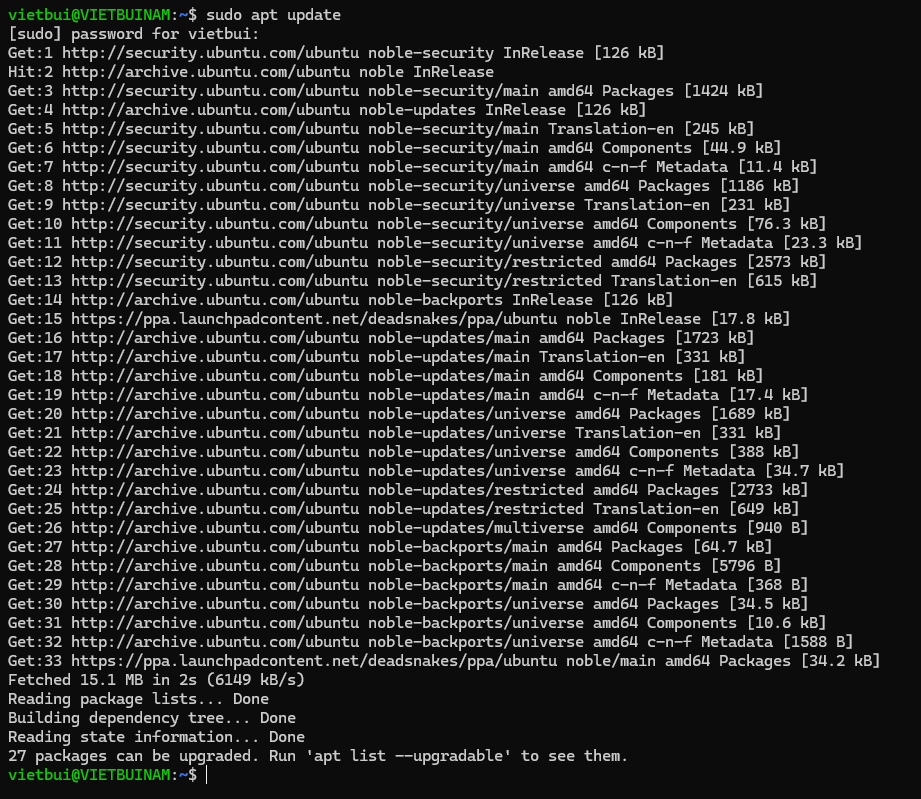
\includegraphics[width=0.75\textwidth]{assets/Screenshot_1.png}
    \caption{System updating on WSL Ubuntu.}
    \label{fig:step1_update_system}
\end{figure}

\begin{figure}[H]
    \centering
    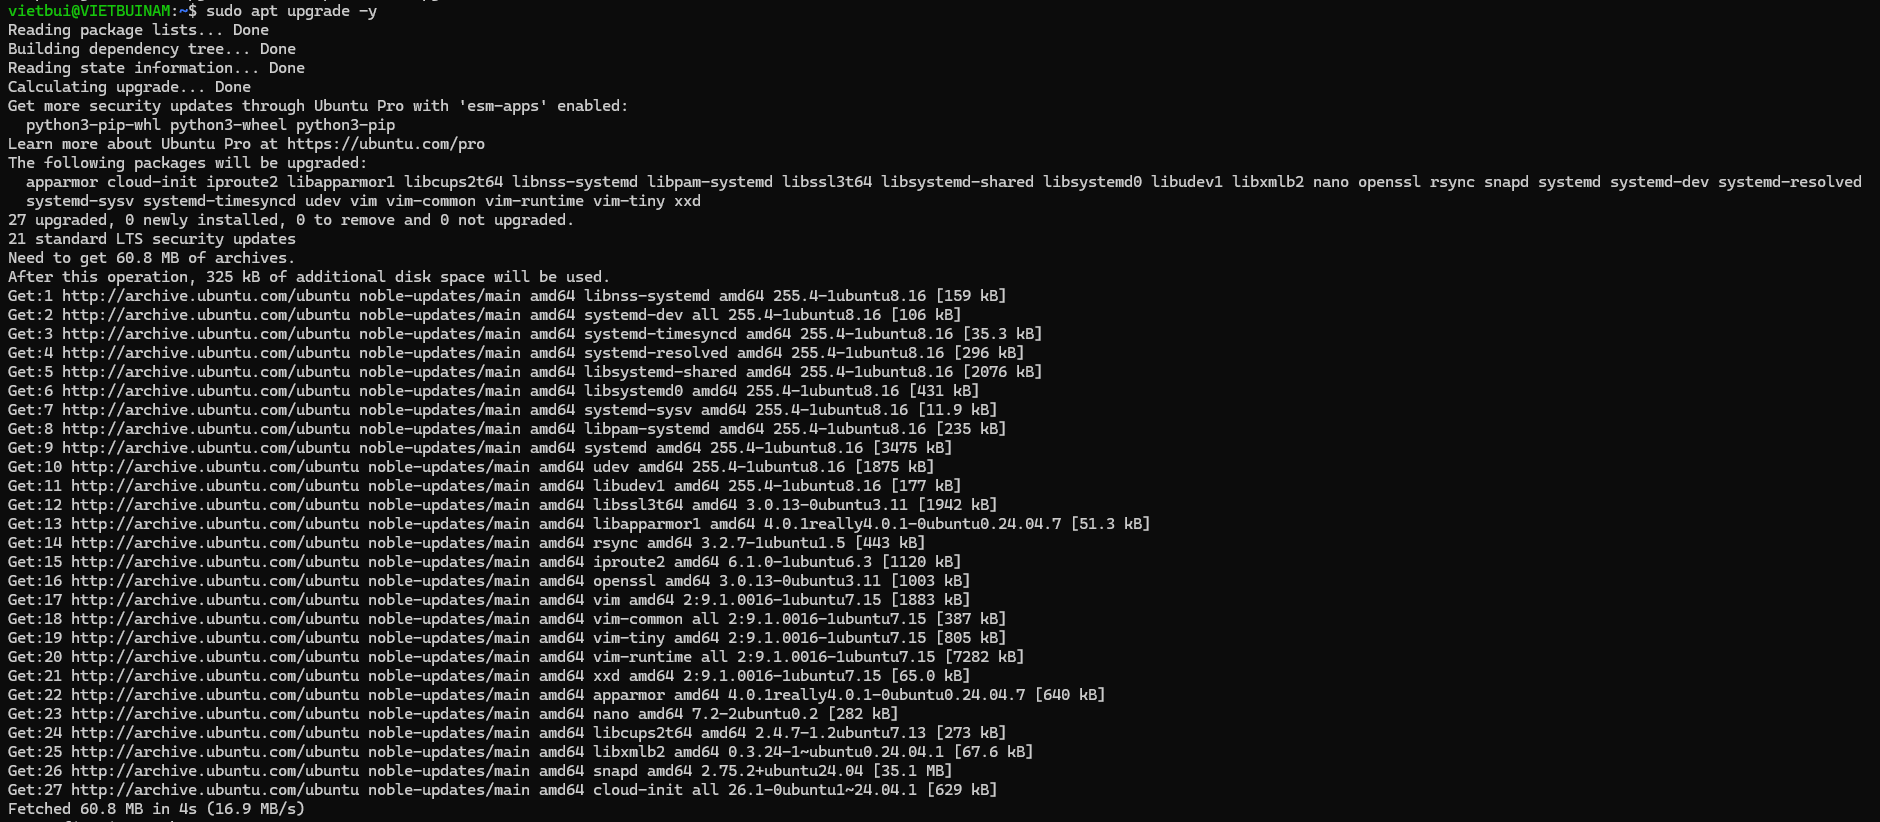
\includegraphics[width=0.75\textwidth]{assets/Screenshot_2.png}
    \caption{System upgrading on WSL Ubuntu.}
    \label{fig:step1_upgrade_system}
\end{figure}

\subsubsection{Step 2: Install Java Development Kit (OpenJDK 17 JDK)}

After the system update, the full OpenJDK 17 JDK package was installed:

\begin{lstlisting}[language=bash]
sudo apt install openjdk-17-jdk -y
\end{lstlisting}

\textit{Explanation:} The \texttt{-y} flag accepts the installation and required dependencies automatically.

\begin{figure}[H]
    \centering
    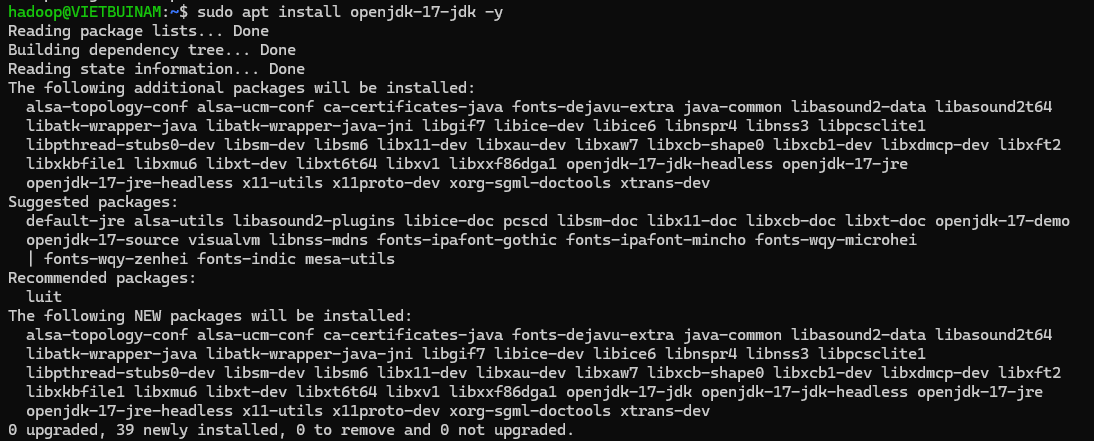
\includegraphics[width=0.75\textwidth]{assets/Screenshot_3.png}
    \caption{Java installation on WSL Ubuntu.}
    \label{fig:step2_install_java}
\end{figure}

\subsubsection{Step 3: Verify installation success (Verification)}

The Java installation was verified by checking the runtime version:

\begin{lstlisting}[language=bash]
java -version
\end{lstlisting}

\begin{figure}[H]
    \centering
    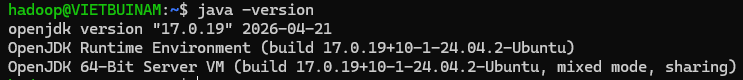
\includegraphics[width=0.75\textwidth]{assets/Screenshot_4.png}
    \caption{Java version verification on WSL Ubuntu.}
    \label{fig:step3_verify_java}
\end{figure}

\begin{itemize}
    \item \textbf{Result:} The system displayed \texttt{openjdk version "17.0.19"} with the 64-Bit Server VM, confirming that Java was installed correctly and ready for Hadoop configuration.
\end{itemize}

\subsection{Creating a Dedicated User and Configuring Passwordless SSH}

Hadoop uses SSH to manage cluster processes, even in pseudo-distributed single-node mode. A dedicated \texttt{hadoop} user was created, and passwordless SSH was configured to support automated service startup.

\subsubsection{Step 1: Create user and grant administrative privileges}

A separate Linux user was created for the Hadoop environment and granted administrative privileges:

\begin{lstlisting}[language=bash]
sudo adduser hadoop
sudo usermod -aG sudo hadoop
\end{lstlisting}

\textit{Explanation:} The first command creates the \texttt{/home/hadoop} account environment. The second command adds the user to the \texttt{sudo} group, allowing administrative commands when required. The session was then switched to the new user using \texttt{sudo su - hadoop}.

\begin{figure}[H]
    \centering
    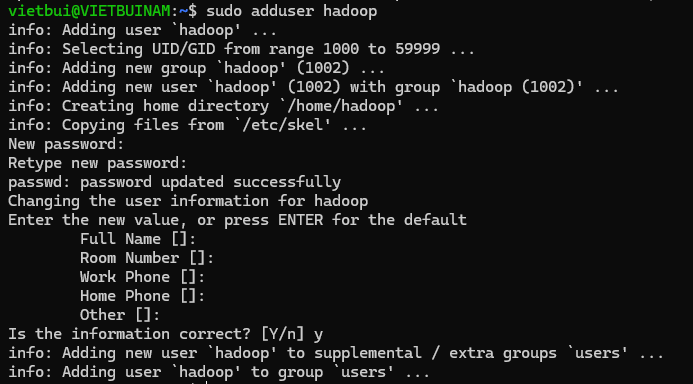
\includegraphics[width=0.75\textwidth]{assets/Screenshot_5.png}
    \caption{Creating a new user in WSL Ubuntu.}
    \label{fig:step1_create_user}
\end{figure}

\begin{figure}[H]
    \centering
    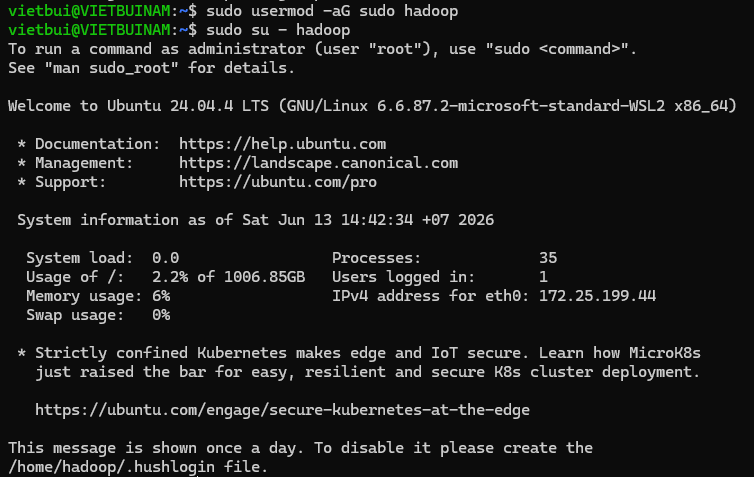
\includegraphics[width=0.75\textwidth]{assets/Screenshot_6.png}
    \caption{Granting sudo privileges and switching to hadoop user workspace.}
    \label{fig:step1_create_user}
\end{figure}

\subsubsection{Step 2: Install OpenSSH service}

The SSH service package was installed to enable secure local communication:

\begin{lstlisting}[language=bash]
sudo apt install ssh
\end{lstlisting}

\begin{figure}[H]
    \centering
    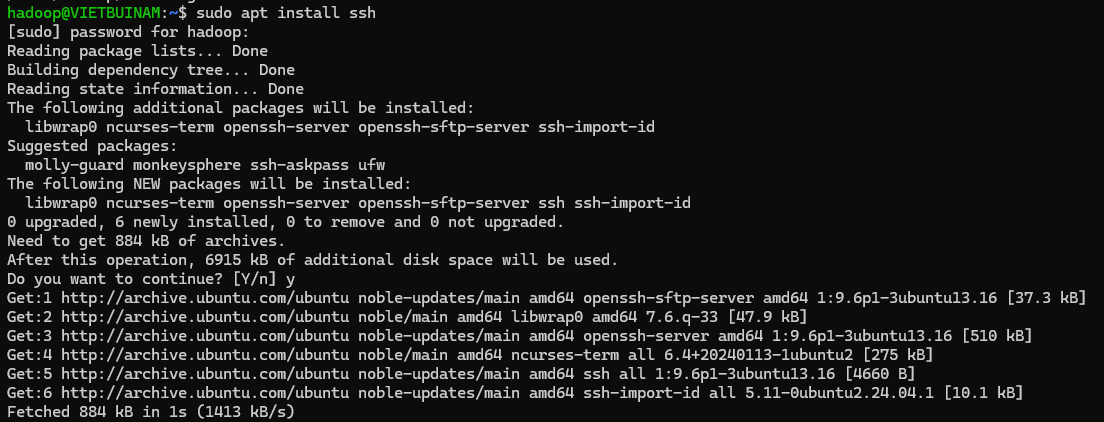
\includegraphics[width=0.75\textwidth]{assets/Screenshot_7.png}
    \caption{Installing OpenSSH service on WSL Ubuntu.}
    \label{fig:step2_install_ssh}
\end{figure}

\subsubsection{Step 3: Generate RSA key pair (SSH Key Generation)}

An RSA key pair was generated for passwordless authentication:

\begin{lstlisting}[language=bash]
ssh-keygen -t rsa
\end{lstlisting}

\textit{Note:} The default key location was used, and the passphrase was left empty so Hadoop services could connect without manual input.

\begin{figure}[H]
    \centering
    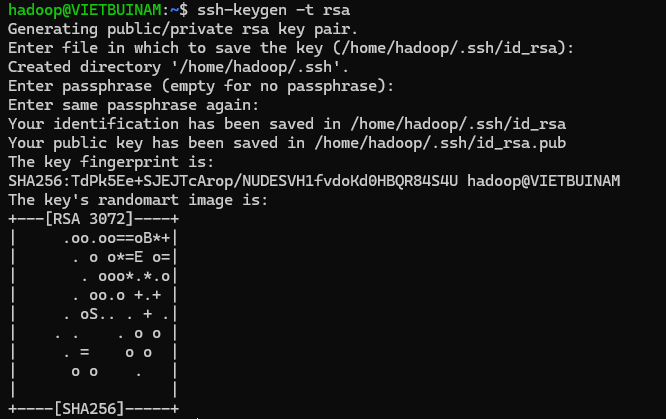
\includegraphics[width=0.75\textwidth]{assets/Screenshot_8.png}
    \caption{Successful RSA key generation with randomart visualization.}
    \label{fig:step3_generate_keys}
\end{figure}

\subsubsection{Step 4: Authorize key and configure file system permissions}

The generated public key was added to \texttt{authorized\_keys}, file permissions were configured, and the SSH service was started:

\begin{lstlisting}[language=bash]
cat ~/.ssh/id_rsa.pub >> ~/.ssh/authorized_keys
sudo chmod 640 ~/.ssh/authorized_keys
sudo service ssh start
\end{lstlisting}

\begin{figure}[H]
    \centering
    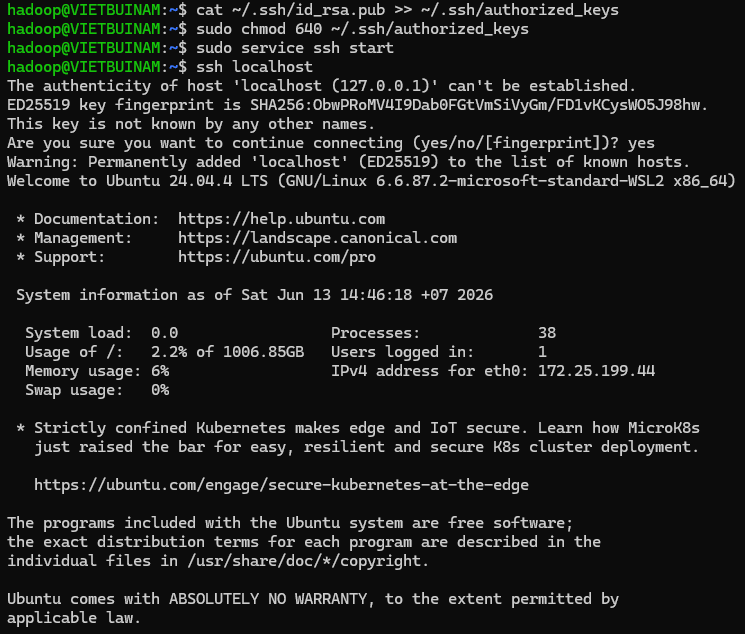
\includegraphics[width=0.75\textwidth]{assets/Screenshot_9.png}
    \caption{Adding the public key to \texttt{authorized\_keys} and starting the SSH service.}
    \label{fig:step4_authorize_key}
\end{figure}

\paragraph{Issue encountered: Incorrect permissions on SSH authorized keys}\

During passwordless SSH configuration, the command

\begin{lstlisting}[language=bash]
sudo chmod 640 ~/.ssh/authorized_keys
\end{lstlisting}

caused the SSH server to reject public-key authentication. Although the mode appeared restrictive, using \texttt{sudo} with \texttt{640} produced an ownership and permission state that SSH did not accept for \texttt{authorized\_keys}.

SSH requires strict ownership and permission settings for both the \texttt{\~{}/.ssh} directory and the \texttt{authorized\_keys} file. If these settings are too permissive or assigned to the wrong owner, the SSH daemon disables public-key authentication for security.

The permissions were corrected under the \texttt{hadoop} account without using \texttt{sudo}:

\begin{lstlisting}[language=bash]
chmod 700 ~/.ssh
chmod 600 ~/.ssh/authorized_keys
\end{lstlisting}

The mode \texttt{700} restricts access to the \texttt{.ssh} directory to the owner, and \texttt{600} restricts \texttt{authorized\_keys} to owner read/write access. After this correction, SSH accepted public-key authentication.

\subsubsection{Step 5: Verify successful Passwordless SSH connection}

The SSH configuration was tested by connecting to localhost:

\begin{lstlisting}[language=bash]
ssh localhost
\end{lstlisting}

\begin{figure}[H]
    \centering
    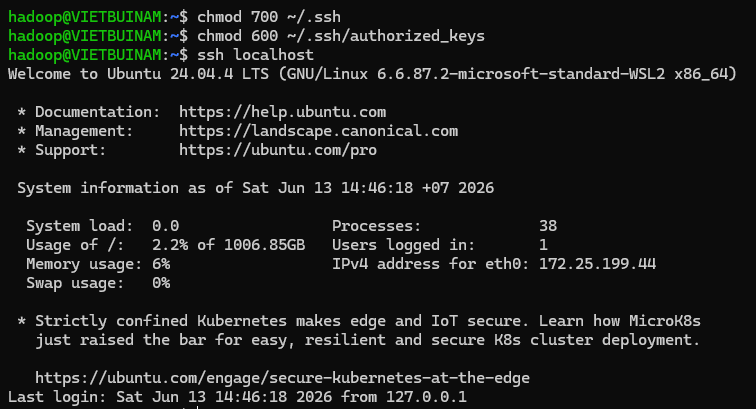
\includegraphics[width=0.75\textwidth]{assets/Screenshot_10.png}
    \caption{Typing \texttt{yes} to confirm the host fingerprint and successful passwordless login.}
    \label{fig:step5_verify_ssh}
\end{figure}

\begin{itemize}
    \item \textbf{Result:} On the first connection, the system displayed a host fingerprint prompt. After entering \texttt{yes}, the host was stored in \texttt{known\_hosts}, and the SSH client logged into \texttt{hadoop@VIETBUINAM} without requesting a password.
\end{itemize}

\subsection{Downloading, Installing, and Configuring Environment Variables for Apache Hadoop}

After Java and SSH were configured, the Apache Hadoop distribution was downloaded and environment variables were set so Hadoop commands could run from any working directory.

\subsubsection{Step 1: Download Apache Hadoop package}

The Hadoop binary distribution was downloaded from the official Apache repository:

\begin{lstlisting}[language=bash]
wget https://downloads.apache.org/hadoop/common/stable/hadoop-3.5.0.tar.gz
\end{lstlisting}

\textit{Explanation:} The file \texttt{hadoop-3.5.0.tar.gz} contains the Hadoop components required for HDFS and YARN in this lab.

\begin{figure}[H]
    \centering
    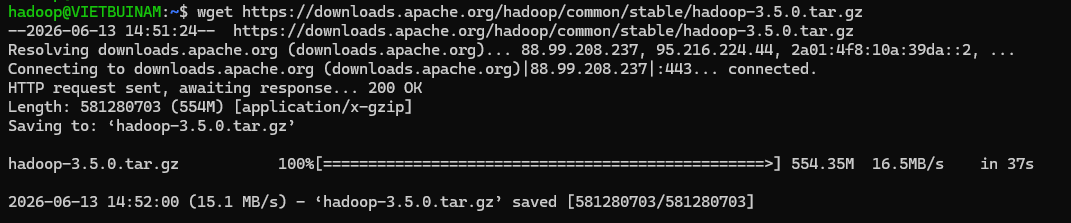
\includegraphics[width=0.75\textwidth]{assets/Screenshot_11.png}
    \caption{Downloading Apache Hadoop package.}
    \label{fig:step1_download_hadoop}
\end{figure}

\subsubsection{Step 2: Extract and organize directory structure}

The downloaded archive was extracted and renamed for simpler path configuration:

\begin{lstlisting}[language=bash]
tar -xzf hadoop-3.5.0.tar.gz
sudo mv hadoop-3.5.0 hadoop
\end{lstlisting}

\textit{Explanation:} \texttt{tar -xzf} extracts the archive, and \texttt{mv} renames the extracted directory to \texttt{hadoop} in the user's home directory.

\begin{figure}[H]
    \centering
    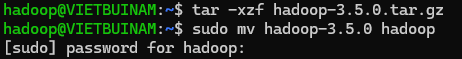
\includegraphics[width=0.75\textwidth]{assets/Screenshot_12.png}
    \caption{Extracting and renaming Hadoop directory.}
    \label{fig:step2_extract_hadoop}
\end{figure}

\subsubsection{Step 3: Assign ownership to target directory}

Ownership of the Hadoop directory was assigned to the dedicated \texttt{hadoop} user:

\begin{lstlisting}[language=bash]
sudo chown -R hadoop:hadoop ~/hadoop
\end{lstlisting}

\textit{Explanation:} The recursive \texttt{-R} option applies ownership to all files and subdirectories, preventing permission errors during service startup.

\begin{figure}[H]
    \centering
    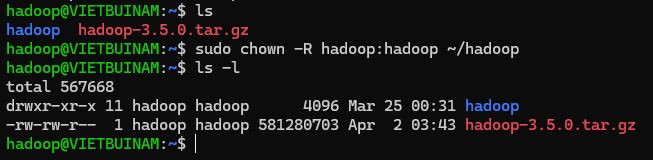
\includegraphics[width=0.75\textwidth]{assets/Screenshot_13.png}
    \caption{Verifying ownership using ls -l showing hadoop:hadoop.}
    \label{fig:step3_verify_ownership}
\end{figure}

\subsubsection{Step 4: Configure environment variables via \texttt{.bashrc}}

The \texttt{.bashrc} file was edited to define Hadoop and Java environment variables:

\begin{lstlisting}[language=bash]
nano ~/.bashrc
\end{lstlisting}

The following configuration was appended to the file:

\begin{lstlisting}[language=bash]
export JAVA_HOME=/usr/lib/jvm/java-17-openjdk-amd64
export HADOOP_HOME=$HOME/hadoop
export HADOOP_INSTALL=$HADOOP_HOME
export HADOOP_MAPRED_HOME=$HADOOP_HOME
export HADOOP_COMMON_HOME=$HADOOP_HOME
export HADOOP_HDFS_HOME=$HADOOP_HOME
export YARN_HOME=$HADOOP_HOME
export HADOOP_COMMON_LIB_NATIVE_DIR=$HADOOP_HOME/lib/native
export PATH=$PATH:$HADOOP_HOME/sbin:$HADOOP_HOME/bin
export HADOOP_OPTS="-Djava.library.path=$HADOOP_HOME/lib/native"
\end{lstlisting}

\begin{figure}[H]
    \centering
    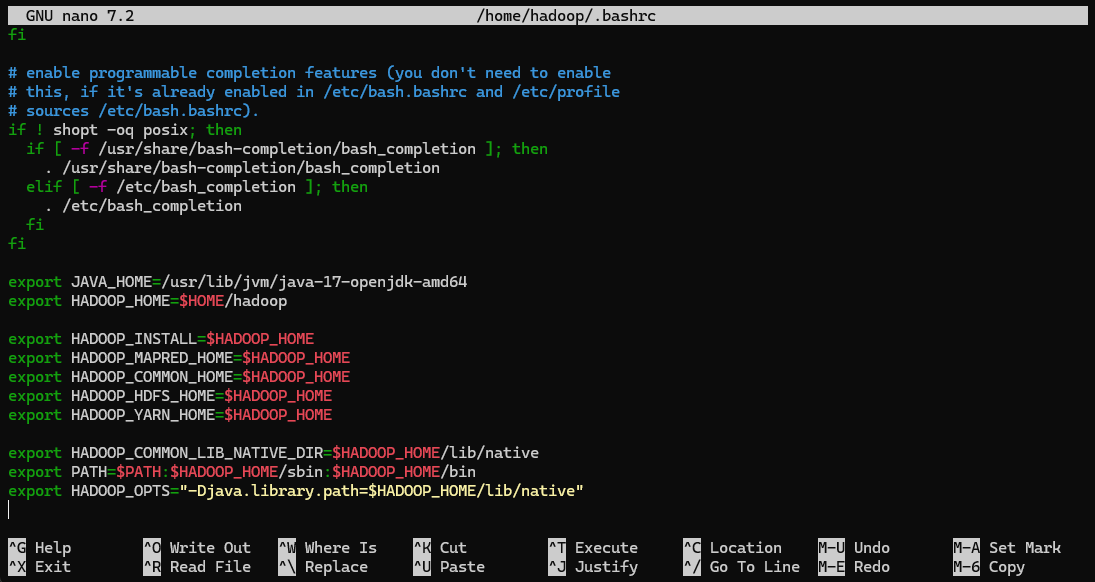
\includegraphics[width=0.75\textwidth]{assets/Screenshot_18.png}
    \caption{Editing .bashrc with Hadoop environment variables in nano.}
    \label{fig:step4_configure_bashrc}
\end{figure}

\subsubsection{Step 5: Activate environment variables}

After saving the file in \texttt{nano}, the current shell session was reloaded:

\begin{lstlisting}[language=bash]
source ~/.bashrc
\end{lstlisting}

\begin{itemize}
    \item \textbf{Result:} The OpenJDK 17 and Apache Hadoop 3.5.0 paths were loaded into the shell environment. Commands such as \texttt{hdfs}, \texttt{hadoop}, and \texttt{start-dfs.sh} can now run from the \texttt{hadoop} user session.
\end{itemize}

\subsection{Configuring Java Path in \texttt{hadoop-env.sh} and System Verification}

Hadoop must reference the Java installation in its internal environment script so HDFS, YARN, and MapReduce services can start consistently.

\subsubsection{Step 1: Set Java path in \texttt{hadoop-env.sh}}

The \texttt{hadoop-env.sh} file in the Hadoop configuration directory was opened:

\begin{lstlisting}[language=bash]
nano $HADOOP_HOME/etc/hadoop/hadoop-env.sh
\end{lstlisting}

The \texttt{JAVA\_HOME} setting was added for the installed OpenJDK 17 path:

\begin{lstlisting}[language=bash]
export JAVA_HOME=/usr/lib/jvm/java-17-openjdk-amd64
\end{lstlisting}

\begin{figure}[H]
    \centering
    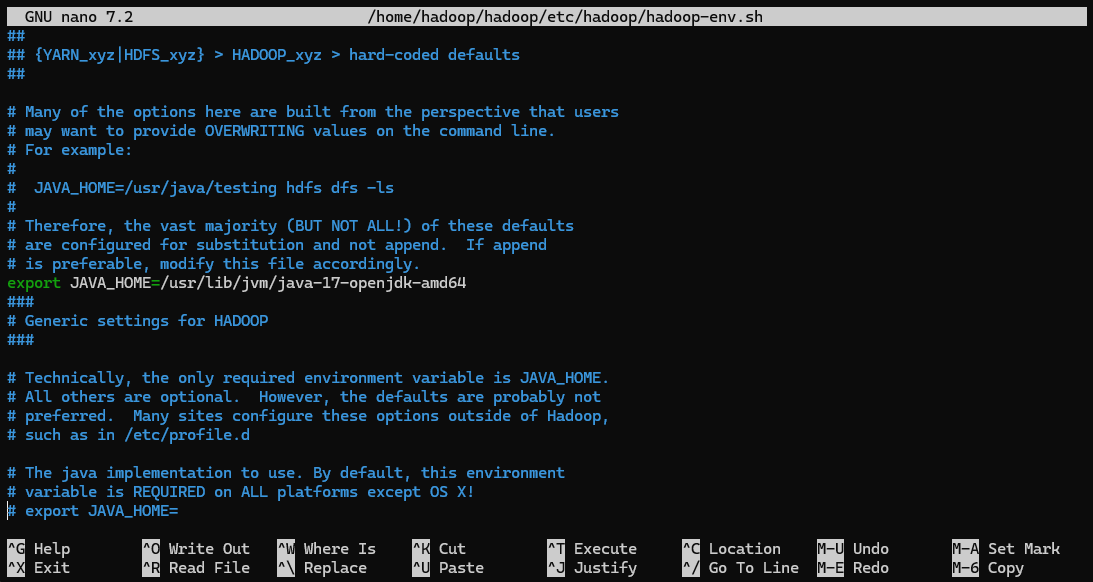
\includegraphics[width=0.75\textwidth]{assets/Screenshot_20.png}
    \caption{Editing hadoop-env.sh with Java path in nano.}
    \label{fig:step5_configure_hadoop_env}
\end{figure}

\subsubsection{Step 2: System version verification}

The Hadoop version command was executed to verify the framework installation and environment configuration:

\begin{lstlisting}[language=bash]
hadoop version
\end{lstlisting}

\begin{figure}[H]
    \centering
    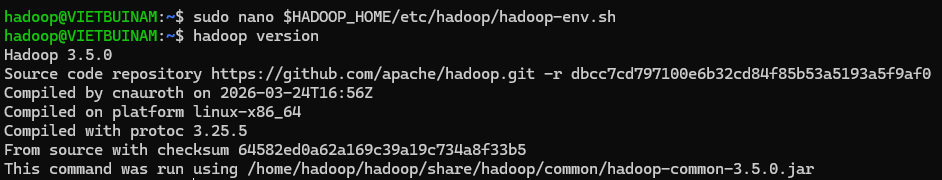
\includegraphics[width=0.75\textwidth]{assets/Screenshot_21.png}
    \caption{Output of hadoop version showing Apache Hadoop 3.5.0 core information.}
    \label{fig:step5_hadoop_version}
\end{figure}

\begin{itemize}
    \item \textbf{Result:} The command returned Hadoop 3.5.0 information and the \texttt{hadoop-common-3.5.0.jar} path, confirming that the base Hadoop environment was configured correctly.
\end{itemize}

\subsection{Configuring Core XML Files and Starting the Single-Node Hadoop Cluster}

Pseudo-distributed mode requires the core Hadoop XML files to define HDFS access, local storage paths, MapReduce execution, and YARN services.

\subsubsection{Step 1: Configure \texttt{core-site.xml}}

\texttt{core-site.xml} was configured to define the default HDFS URI and communication port:

\begin{lstlisting}[language=bash]
nano $HADOOP_HOME/etc/hadoop/core-site.xml
\end{lstlisting}

\textit{Inserted property:} The default URI was set to \texttt{hdfs://localhost:9000}.

\begin{figure}[H]
    \centering
    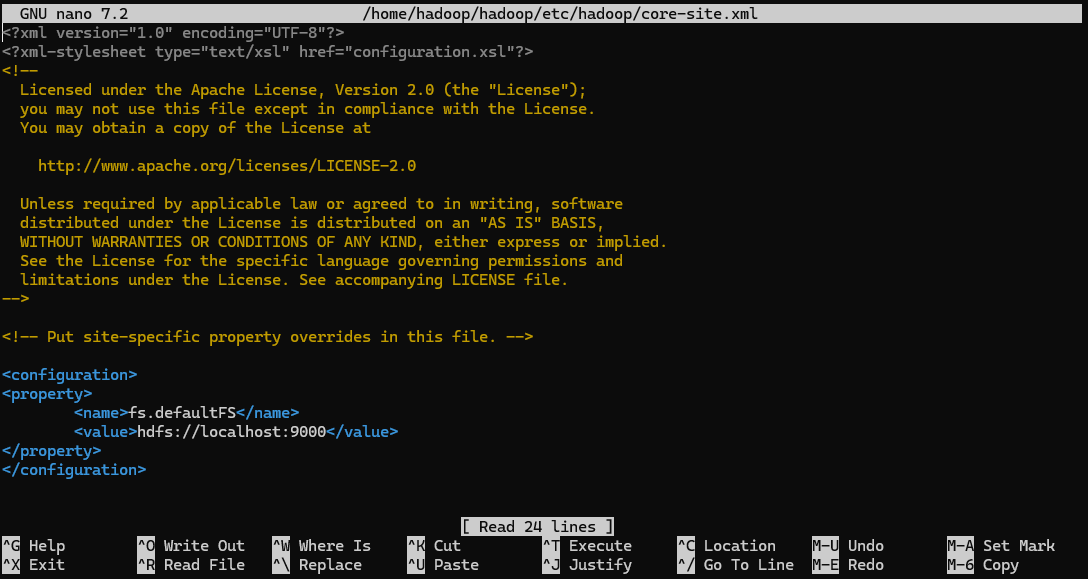
\includegraphics[width=0.75\textwidth]{assets/Screenshot_22.png}
    \caption{Configuring default filesystem property in core-site.xml.}
    \label{fig:step5_core_site}
\end{figure}

\subsubsection{Step 2: Configure \texttt{hdfs-site.xml}}

Local directories were created for NameNode metadata and DataNode block storage, then added to \texttt{hdfs-site.xml}:

\begin{lstlisting}[language=bash]
mkdir -p /home/hadoop/hdfs/{namenode,datanode}
nano $HADOOP_HOME/etc/hadoop/hdfs-site.xml
\end{lstlisting}

\begin{figure}[H]
    \centering
    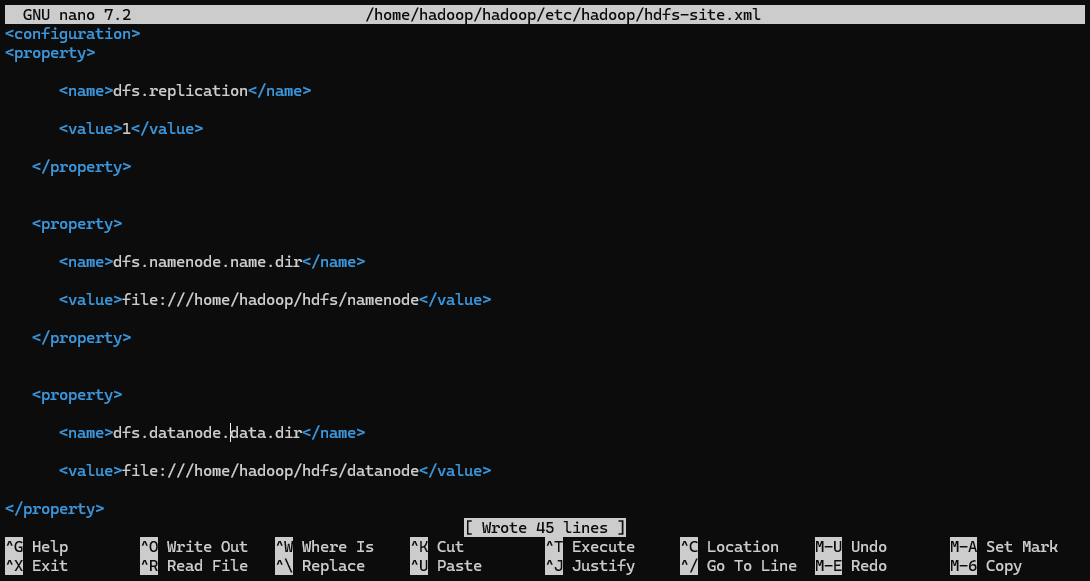
\includegraphics[width=0.75\textwidth]{assets/Screenshot_23.png}
    \caption{Configuring HDFS storage directories and replication factor.}
    \label{fig:step5_hdfs_site}
\end{figure}

\textit{Inserted properties:} The replication factor \texttt{dfs.replication} was set to $1$ for the single-node setup, and the NameNode and DataNode storage paths were set to the created directories.

\subsubsection{Step 3: Configure \texttt{mapred-site.xml} and \texttt{yarn-site.xml}}

MapReduce was configured to use YARN for job scheduling and resource management:

\begin{lstlisting}[language=bash]
nano $HADOOP_HOME/etc/hadoop/mapred-site.xml
nano $HADOOP_HOME/etc/hadoop/yarn-site.xml
\end{lstlisting}

\textit{Inserted properties:} In \texttt{mapred-site.xml}, the execution framework was set to \texttt{yarn}. In \texttt{yarn-site.xml}, \texttt{mapreduce\_shuffle} was enabled to support the MapReduce Shuffle \& Sort phase.

\begin{figure}[H]
    \centering
    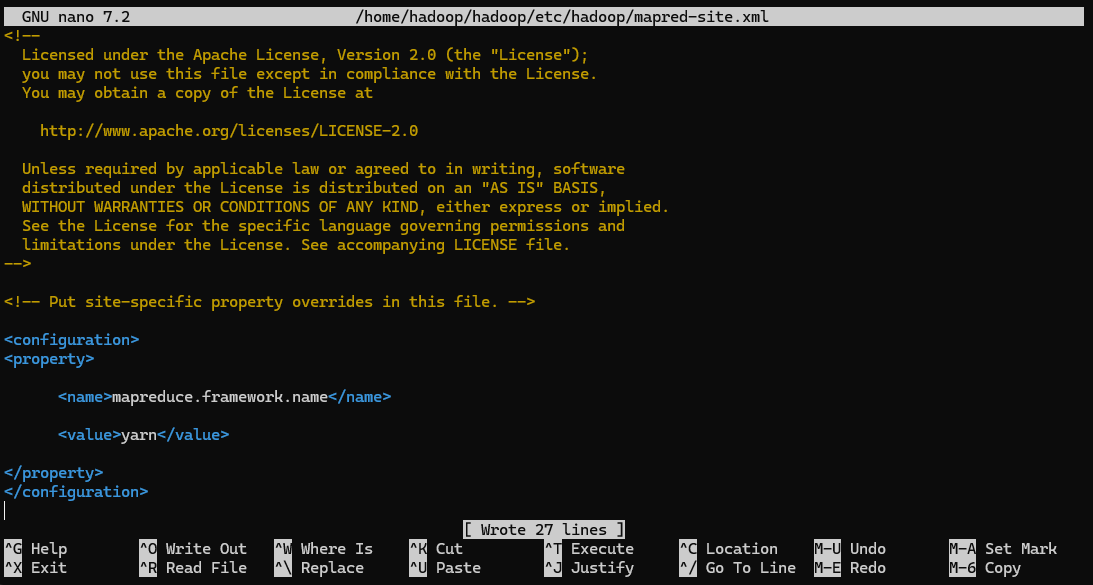
\includegraphics[width=0.75\textwidth]{assets/Screenshot_24.png}
    \caption{Configuring YARN framework in mapred-site.xml.}
    \label{fig:step5_mapred_site}
\end{figure}

\begin{figure}[H]
    \centering
    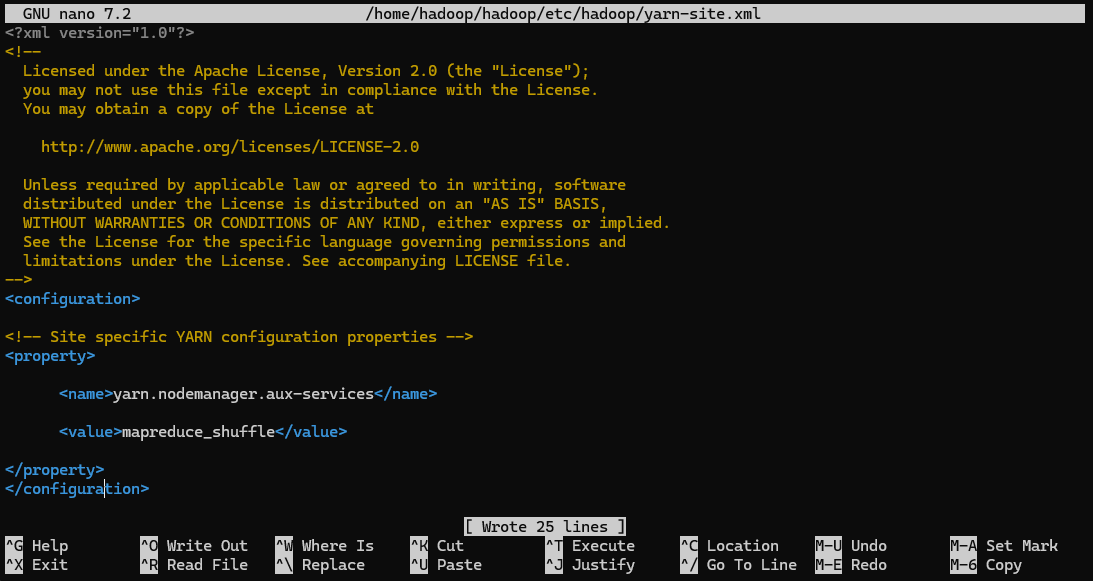
\includegraphics[width=0.75\textwidth]{assets/Screenshot_25.png}
    \caption{Enabling NodeManager shuffle service in yarn-site.xml.}
    \label{fig:step5_yarn_site}
\end{figure}

\subsubsection{Step 4: Format the NameNode (HDFS Format)}

Before the first cluster startup, the NameNode was formatted to initialize HDFS metadata:

\begin{lstlisting}[language=bash]
hdfs namenode -format
\end{lstlisting}

\begin{figure}[H]
    \centering
    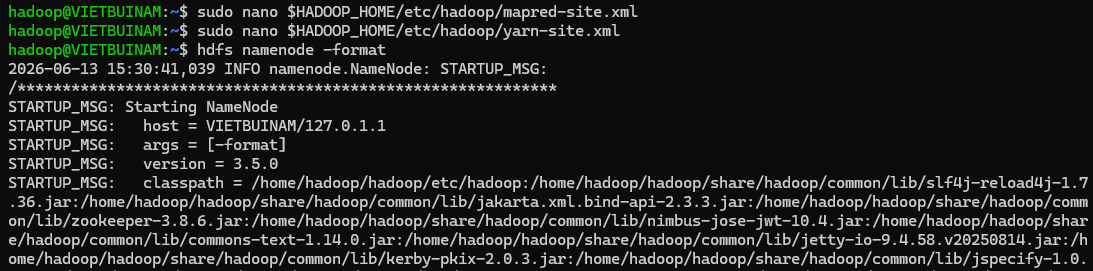
\includegraphics[width=0.75\textwidth]{assets/Screenshot_26.png}
    \caption{Formatting the NameNode metadata storage.}
    \label{fig:step5_namenode_format}
\end{figure}

\subsubsection{Step 5: Start all services and verify system status}

The startup scripts were executed, and Java processes were checked to verify the cluster status:

\begin{lstlisting}[language=bash]
start-dfs.sh
start-yarn.sh
jps
\end{lstlisting}

\begin{figure}[H]
    \centering
    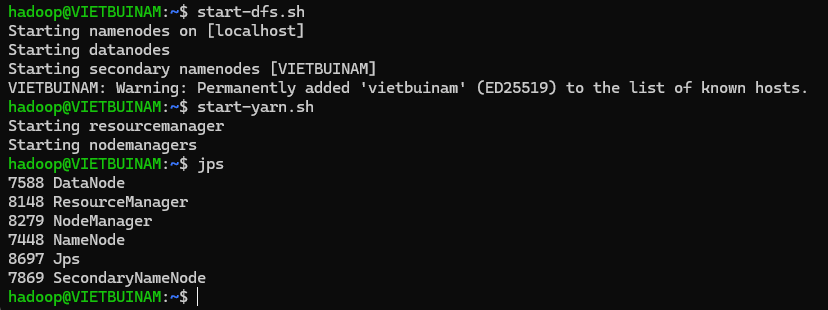
\includegraphics[width=0.75\textwidth]{assets/Screenshot_27.png}
    \caption{Successfully starting HDFS, YARN and jps showing all core processes.}
    \label{fig:step5_start_services}
\end{figure}

\begin{itemize}
    \item \textbf{Result:} The \texttt{jps} output showed \textbf{NameNode}, \textbf{SecondaryNameNode}, \textbf{DataNode}, \textbf{ResourceManager}, and \textbf{NodeManager} running under separate PIDs. This confirms that the pseudo-distributed Hadoop cluster was started successfully.
\end{itemize}

\subsection{Cluster Status Verification via Web UI}

Hadoop Web UI pages were used to confirm the HDFS and YARN status after startup.

\subsubsection{Step 1: Explore NameNode Web UI}

The NameNode Web UI was opened at \texttt{http://localhost:9870} to inspect HDFS status.

\begin{figure}[H]
    \centering
    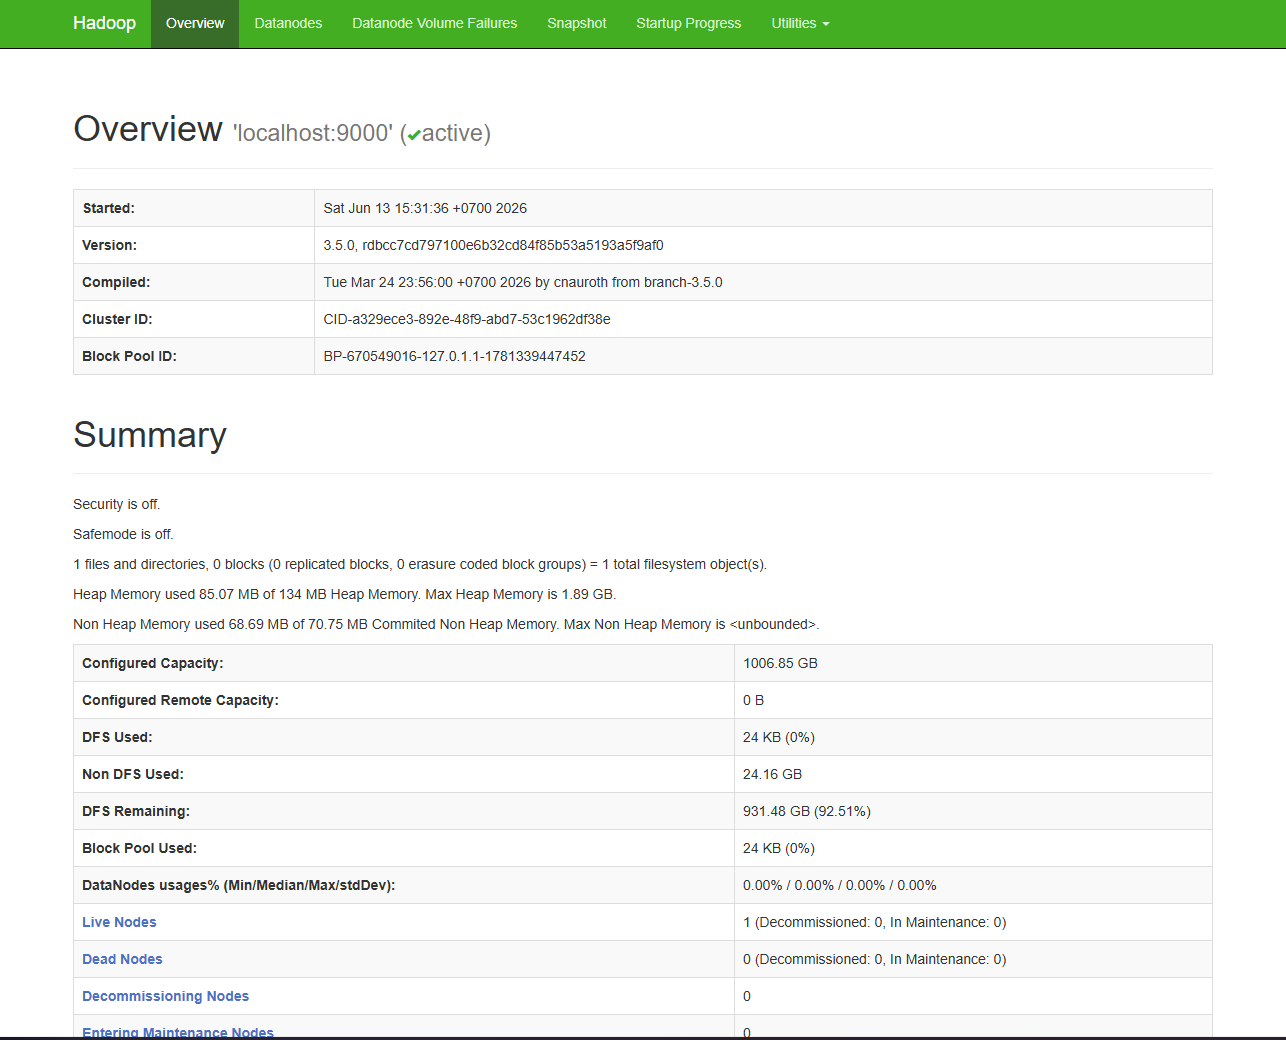
\includegraphics[width=0.7\textwidth]{assets/Screenshot_28.png}
    \caption{NameNode Web UI showing cluster status.}
    \label{fig:namenode_webui}
\end{figure}

\begin{itemize}
    \item \textbf{System Metrics Analysis:}
    \begin{itemize}
        \item \textbf{State:} The interface showed the NameNode state as \texttt{active} and reported Hadoop version \texttt{3.5.0}, matching the installed environment.
        \item \textbf{Summary:} The status \texttt{Safemode is off} indicates that HDFS is ready for read/write operations. The \texttt{Live Nodes} value was \textbf{1}, confirming that the single DataNode was connected, and \texttt{DFS Remaining} was $92.51\%$.
    \end{itemize}
\end{itemize}

\subsubsection{Step 2: Explore YARN ResourceManager Web UI}

The ResourceManager Web UI was opened at \texttt{http://localhost:8088} to inspect YARN status.

\begin{figure}[H]
    \centering
    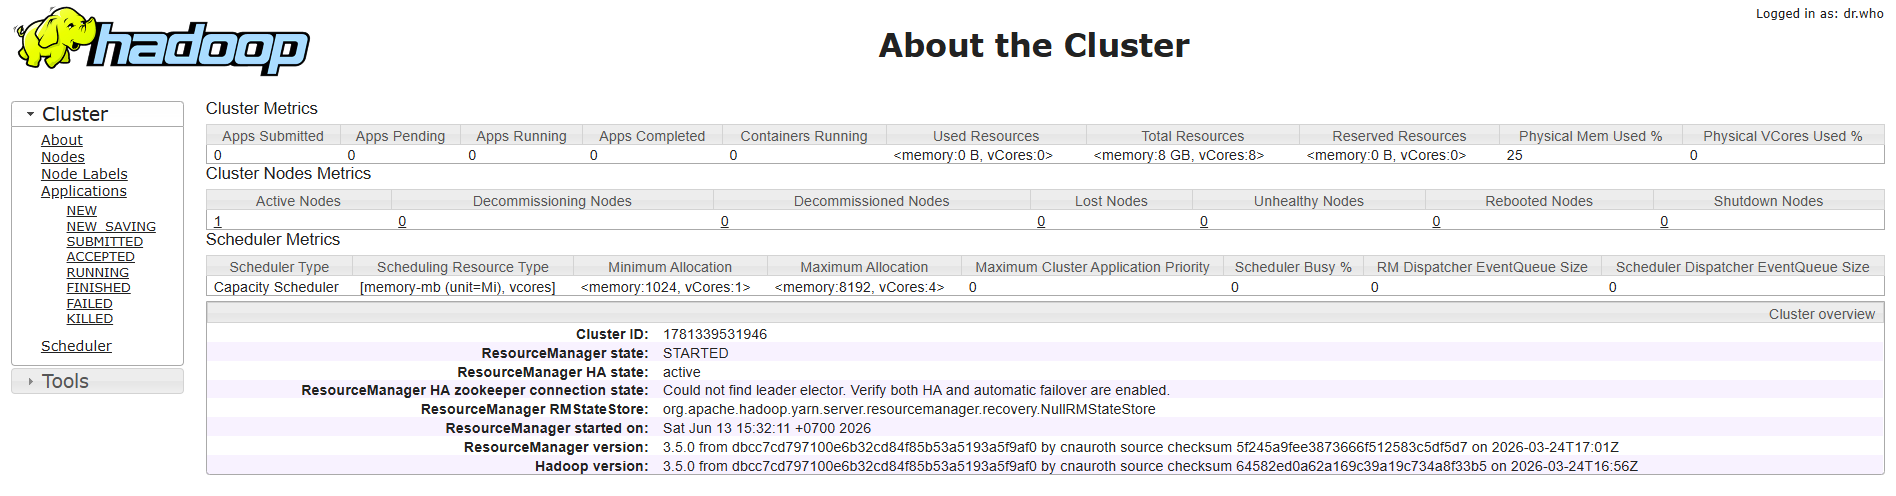
\includegraphics[width=0.75\textwidth]{assets/Screenshot_29.png}
    \caption{YARN ResourceManager Web UI showing cluster metrics and scheduler information.}
    \label{fig:yarn_resourcemanager}
\end{figure}

\begin{itemize}
    \item \textbf{System Metrics Analysis:}
    \begin{itemize}
        \item \textbf{Cluster Metrics:} \texttt{Apps Running} and \texttt{Apps Completed} were both \textbf{0} because no processing jobs had been submitted. The \texttt{Active Nodes} value was \textbf{1}, indicating that the NodeManager was available for containers.
        \item \textbf{Total Resources:} The interface reported \texttt{8 GB} virtual memory and \texttt{8 vCores}. The \texttt{ResourceManager HA state} was \texttt{active}, confirming that the scheduler was initialized.
    \end{itemize}
    \item \textbf{Conclusion:} The Web UI metrics matched the local process verification, confirming that the cluster was ready for HDFS operations through the CLI.
\end{itemize}

\section{Pseudo-Distributed Mode}

\subsection{Step 1: Creating the System Directory and Dedicated User}

\begin{itemize}
    \item \textbf{Create the root directory:} The parent directory \texttt{/hcmus} was created on HDFS as the common storage workspace:
\end{itemize}

\begin{lstlisting}[language=bash]
hdfs dfs -mkdir /hcmus
\end{lstlisting}

\begin{itemize}
    \item \textbf{Create a dedicated system user:} A Linux user named \texttt{khtn\_23127516} was created for ownership assignment:
\end{itemize}

\begin{lstlisting}[language=bash]
sudo adduser khtn_23127516
\end{lstlisting}

\begin{figure}[H]
    \centering
    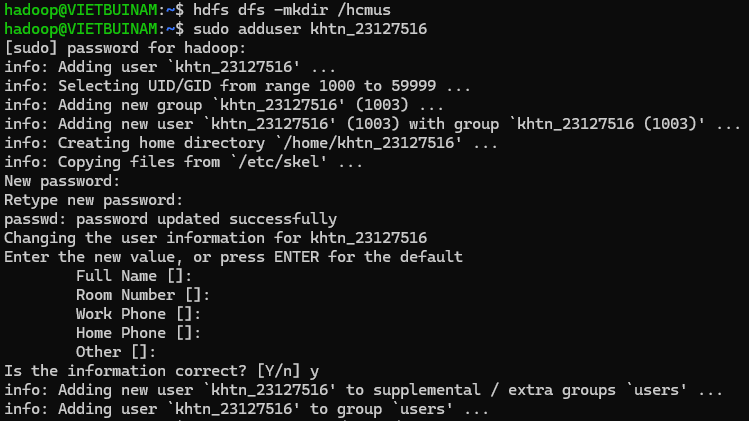
\includegraphics[width=0.75\textwidth]{assets/Screenshot_30.png}
    \caption{Creating the root directory \texttt{/hcmus} and configuring the user \texttt{khtn\_23127516}.}
    \label{fig:hdfs_setup}
\end{figure}

\subsection{Step 2: Managing Subdirectories, Uploading Data, and Configuring Permissions}

\begin{itemize}
    \item \textbf{Create the student directory:} The subdirectory \texttt{/hcmus/23127516} was created under the HDFS root directory hierarchy.

    \item \textbf{Upload data to HDFS:} A local text file named \texttt{sample.txt} was created and uploaded to HDFS:
\end{itemize}

\begin{lstlisting}[language=bash]
echo "HDFS Test File" > sample.txt
hdfs dfs -put sample.txt /hcmus/23127516/
\end{lstlisting}

\begin{itemize}
    \item \textbf{Configure permissions and transfer ownership:} Permission mode \texttt{744} was assigned, and ownership of the student directory was transferred to \texttt{khtn\_23127516}:
\end{itemize}

\begin{lstlisting}[language=bash]
hdfs dfs -chmod 744 /hcmus/23127516
hdfs dfs -chown khtn_23127516 /hcmus/23127516
\end{lstlisting}

\begin{figure}[H]
    \centering
    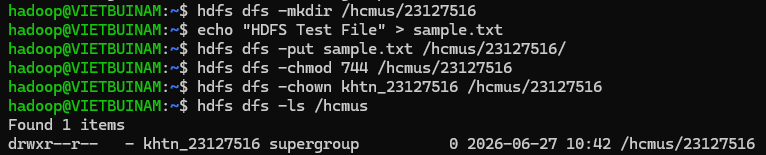
\includegraphics[width=0.75\textwidth]{assets/Screenshot_31.png}
    \caption{Executing data operations, applying \texttt{chmod 744}, and verifying the directory structure using the \texttt{ls} command.}
    \label{fig:hdfs_verification}
\end{figure}

\begin{itemize}
    \item \textbf{Verification:} The command \texttt{hdfs dfs -ls /hcmus} confirmed the expected state. The directory showed permission attribute \texttt{drwxr--r--}, corresponding to mode \texttt{744}, and ownership was assigned to \texttt{khtn\_23127516}.
\end{itemize}

\subsection{Step 3: Executing the JAR Program for Automated System Verification}

The verification JAR was executed from \texttt{/home/hadoop/run} to validate the HDFS configuration automatically.

\begin{itemize}
    \item \textbf{Execution command:}
\end{itemize}

\begin{lstlisting}[language=bash]
mkdir -p ~/run && cd ~/run
java -jar ~/hadoop-test.jar 9000 /hcmus/23127516
\end{lstlisting}

\begin{figure}[H]
    \centering
    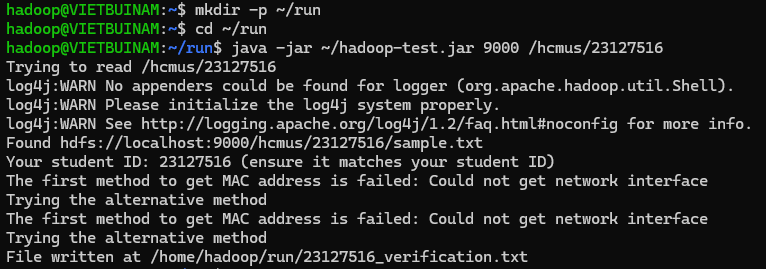
\includegraphics[width=0.75\textwidth]{assets/Screenshot_32.png}
    \caption{Successful execution of \texttt{hadoop-test.jar} generating the verification code.}
    \label{fig:verification_results}
\end{figure}

\section{Word Count}

\subsection{Step 1: Creating the HDFS Directory Structure and Uploading the Input Dataset}

The HDFS input directory was created, and \texttt{words.txt} was uploaded for the Word Count job.

\textbf{Commands executed:}

\begin{lstlisting}[language=bash]
hdfs dfs -mkdir -p /hcmus/23127516/warmup/input
hdfs dfs -put -f words.txt /hcmus/23127516/warmup/input/
hdfs dfs -ls /hcmus/23127516/warmup/input
\end{lstlisting}

\begin{figure}[H]
    \centering
    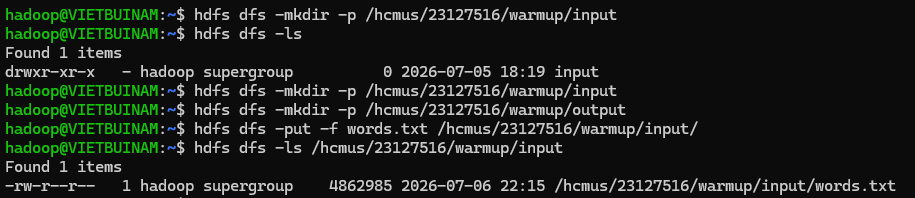
\includegraphics[width=0.75\textwidth]{assets/Screenshot_33.png}
    \caption{Creating the HDFS directory structure and uploading the input dataset \texttt{words.txt}.}
    \label{fig:hdfs_wordcount_setup}
\end{figure}

\subsection{Step 2: Compiling the Scala Application}

\texttt{WordCount.scala} was compiled with the Hadoop classpath and packaged into \texttt{WordCount.jar}.

\textbf{Commands executed:}

\begin{lstlisting}[language=bash]
scalac -classpath "$(hadoop classpath)" WordCount.scala
jar cvf WordCount.jar WordCount*.class
\end{lstlisting}

\begin{figure}[H]
    \centering
    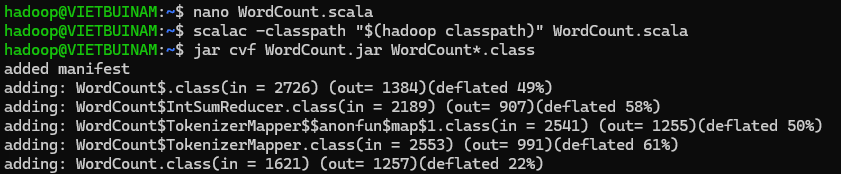
\includegraphics[width=0.75\textwidth]{assets/Screenshot_34.png}
    \caption{Successful compilation and packaging of the Scala application into a JAR file.}
    \label{fig:scala_compilation}
\end{figure}

%------------------------------------------------

\subsection{Step 3: Submitting the Job to YARN and Resolving the \texttt{ClassNotFoundException}}

The first MapReduce submission failed inside the YARN containers with the following exception:
\begin{quote}
\texttt{Error: java.lang.ClassNotFoundException: scala.Function1}
\end{quote}

\begin{figure}[H]
    \centering
    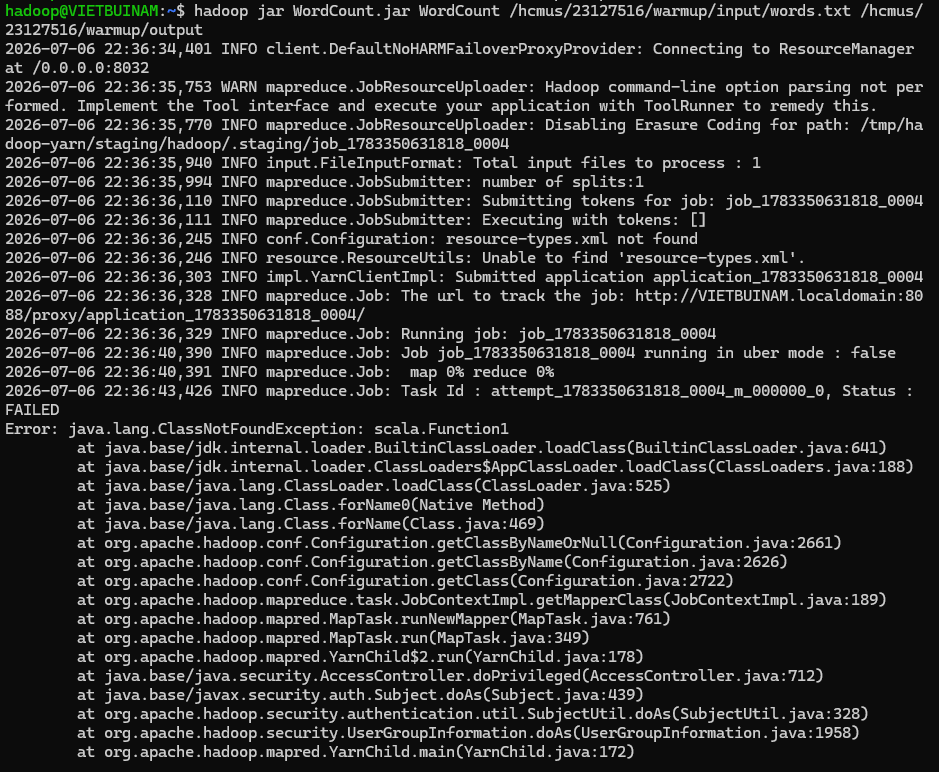
\includegraphics[width=0.7\textwidth]{assets/Screenshot_35.png}
    \caption{System log reporting the missing Scala runtime library.}
    \label{fig:missing_scala_library}
\end{figure}

\textbf{Analysis}

The \texttt{hadoop jar} command loaded the Hadoop libraries, but the YARN container JVMs did not include the Scala runtime. As a result, the containers could not find \texttt{scala.Function1}, which is provided by \texttt{scala-library.jar}, and the Mapper tasks failed.

\textbf{Solution}

The Scala runtime path \texttt{/usr/share/scala-2.11/lib/*} was added to \texttt{yarn.application.classpath} in \texttt{yarn-site.xml}. The incomplete output directory was then removed, and YARN was restarted to apply the configuration.

\textbf{Commands executed:}

\begin{lstlisting}[language=bash]
nano $HADOOP_HOME/etc/hadoop/yarn-site.xml
\end{lstlisting}

\begin{figure}[H]
    \centering
    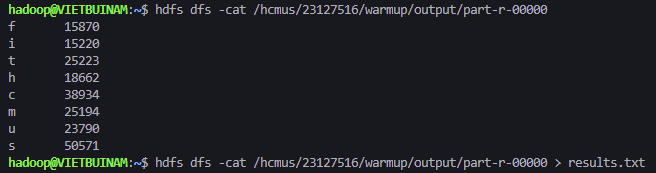
\includegraphics[width=0.75\textwidth]{assets/Screenshot_39.png}
    \caption{Adding the Scala runtime library path to the YARN classpath in \texttt{yarn-site.xml}.}
    \label{fig:yarn_classpath_update}
\end{figure}

\begin{lstlisting}[language=bash]
hdfs dfs -rm -r -f /hcmus/23127516/warmup/output
stop-yarn.sh && start-yarn.sh
\end{lstlisting}

\begin{figure}[H]
    \centering
    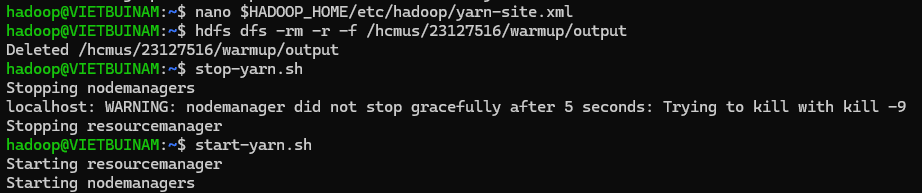
\includegraphics[width=0.75\textwidth]{assets/Screenshot_36.png}
    \caption{Removing the incomplete output directory and restarting the YARN cluster.}
    \label{fig:yarn_restart}
\end{figure}

%------------------------------------------------

\subsection{Step 4: Successful Job Execution}

After the YARN classpath was updated, the MapReduce application was submitted again.

\textbf{Command executed:}

\begin{lstlisting}[language=bash]
hadoop jar WordCount.jar WordCount \
/hcmus/23127516/warmup/input/words.txt \
/hcmus/23127516/warmup/output
\end{lstlisting}

\begin{figure}[H]
    \centering
    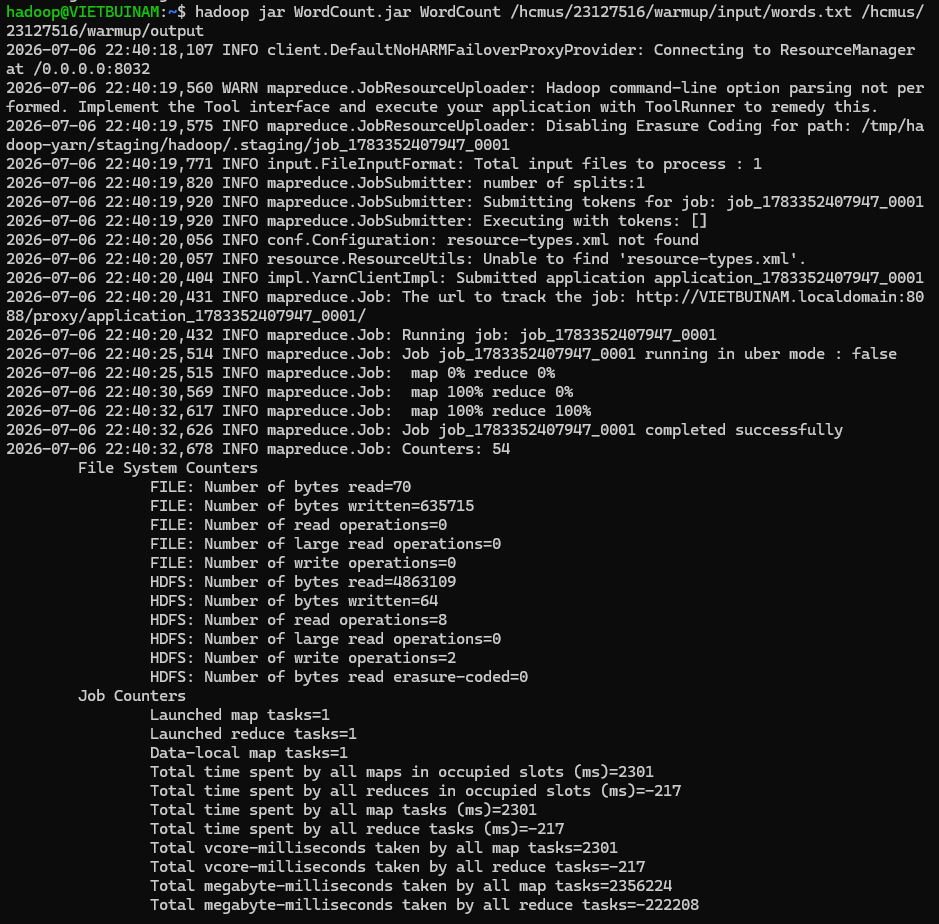
\includegraphics[width=0.75\textwidth]{assets/Screenshot_37.png}
    \caption{Successful completion of the MapReduce job (map 100\%, reduce 100\%).}
    \label{fig:successful_execution}
\end{figure}

\textbf{Result}

The MapReduce job completed successfully. The HDFS output was exported to the local machine as the TSV-formatted file \texttt{results.txt}.

\begin{figure}[H]
    \centering
    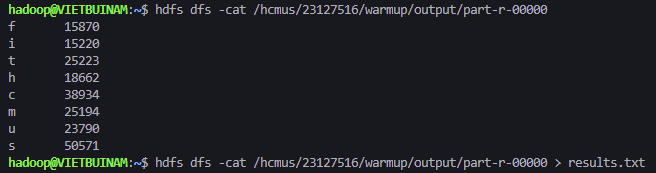
\includegraphics[width=0.75\textwidth]{assets/Screenshot_39.png}
    \caption{Exporting the output results.}
    \label{fig:results_export}
\end{figure}
\end{document}
